\chapter{Momentum Transport}

\section{基本数学知识}
\subsection{大学白学了}

\[\frac{d}{dx}(uv) = u\frac{dv}{dx} + v\frac{du}{dx}\]

\subsection{矢量计算}

几个基本的等式:

\[\nabla s = \frac{\partial s}{\partial x}\bm{i} +  \frac{\partial s}{\partial y}\bm{j} + \frac{\partial s}{\partial z}\bm{k}\]

\[\nabla\cdot\bm{u} = \frac{\partial u}{\partial x} + \frac{\partial v}{\partial y} + \frac{\partial w}{\partial z}\]

\[\nabla^2\bm{u} = \frac{\partial^2 u}{\partial x^2} + \frac{\partial^2 v}{\partial y^2} + \frac{\partial^2 w}{\partial z^2} \]

\[\nabla\cdot (s\mathbf{u}) = s\nabla\cdot\bm{u}+\bm{u}\cdot\nabla s\]

\subsection{Gauss散度定理}
整个控制体内的源汇项=控制体表面的净通量:

\begin{equation}\label{Gauss}
\int_{V}(\nabla\cdot \bm{u})dV = \int_{S} (\bm{u\cdot n})dS
\end{equation}

\subsection{Leibniz积分法则}

给出了一个对积分变量为函数的积分求导的法则,右侧第一项解释了积分随时间的变化,二三两项区域内物理量的得失。

\begin{equation}
    \frac{d}{dt} \int_{a(t)}^{b(t)} \phi(x,t) dx = \int_{a(t)}^{b(t)} \frac{\partial \phi}{\partial t} dx + \phi(b(t),t) \frac{\partial b}{\partial t} - \phi(a(t),t)\frac{\partial a}{\partial t}
\end{equation}

对由面$ S(t) $包围的封闭三维空间$ V(t) $来讲,假设面的移动速度为$ \mathbf{v_s} $,有如下积分法则:

\begin{equation}
    \frac{d}{dt} \int_{V(t)} \phi dV = \int_{V(t)} \frac{\partial \phi}{\partial t} dV + \int_{S(t)} \phi(\mathbf{v_s}\cdot \mathbf{n}) dS
\end{equation}

若控制体不移动,则:

\begin{equation}\label{Leibniz}
\frac{d}{dt} \int_{V(t)} \phi dV = \int_{V(t)} \frac{\partial \phi}{\partial t} dV
\end{equation}


\section{无量纲数}\label{dimensionless-number}

Reynolds Number,定义为惯性力和粘性力的比:

\[ Re = \frac{\rho UL}{\mu} \]

Grashof Number,定义为浮力和粘性力的比,$ \nu $为动力粘度:

\[ Gr = \frac{g\beta\Delta TL^3}{\nu^2} \]

P\'{e}clet Number,定义为对流传递速率与扩散传递速率之比,$ D $为质量扩散系数:

\[ Pe =
\begin{cases}
\frac{\rho ULc_p}{k} = \frac{UL}{\alpha} = RePr & \text{for heat transfer}\\
\frac{UL}{D} = ReSc & \text{for mass transfer}
\end{cases}
\]

Prandtl Number,定义为动量扩散率和热扩散率之比(也代表流动边界层和热边界层之比),$ k $为导热系数,$ \alpha $为热扩散系数,$ \nu $为动力粘度($ \nu = \mu/\rho $)。$ Pr<1 $时,热边界层比速度边界层厚;$ Pr>1 $,热边界层比速度边界层薄。

气体的$ Pr\approx 1 $,意味着流体中动量和能量传递速率相同;如果流体的$ Pr\ll 1 $(比如液态金属),能量传递比动量传递快;如果流体的$ Pr \gg 1 $(比如油),其能量传递比质量传递慢。这可以理解层热边界层与动量边界层厚度不一致所引起的现象。

\[ Pr = \frac{\mu c_p}{k} = \frac{\mu/\rho}{k/\rho c_p} = \frac{\nu}{\alpha} \]

Schmidt Number,定义为动量扩散率和质量扩散率之比,用于描述同时存在动量和质量扩散过程的流体流动。$ Sc $在质量传递中的作用与$ Pr $在能量传递中的作用类似,物理意义上表示速度边界层与传质边界层的相对厚度。$ Sc<1 $时,传质边界层比速度边界层厚;$ Sc>1 $时,传质边界层比速度边界层薄。

\[ Sc = \frac{\nu}{D} = \frac{\mu}{\rho D} \]

Lewis Number,定义为热扩散系数与质量扩散系数之比,系统涉及到质量和能量的同时传递:

\[Le = \frac{\alpha}{D} = \frac{Sc}{Pr}\]

Nusselt Number,定义为对流和热传导之比:

\[Nu = \frac{hL}{k}\]

Sherwood number,定义为分子质量传递阻力与对流质量传递阻力之比,其中$ h $为对流传质系数(\si{\meter\per\second}):

\[Sh = \frac{hL}{D}\]

Mach Number,定义为速度和介质中声速之比:

\[ M = \frac{|\mathbf{v}|}{a} \]

声速由下式计算,其中$ \gamma=c_p/c_v $为比气体常数:

\[a=\sqrt{\gamma\left( \frac{\partial p}{\partial \rho} \right)_T}\]

对理想气体而言,简化如下:

\[a=\sqrt{\gamma RT}\]

Eckert Number,动能和焓之比。如果$ Ec\ll 1 $,能量方程中的粘性耗散和压力功就可以忽略(事实上这个无量纲数就是为了表明,在速度不太高的情况下,可压缩流体的的粘性耗散和压力功可以忽略):

\[Ec=\frac{\mathbf{v\cdot v}}{c_p\Delta T}\]

Froude number,定义为特征速度和重力波速度之比,用来表征固体在流体中运动的情况,$ Fr $越高意味着固体所受阻力越大:

\[Fr = \frac{U}{\sqrt{gL}}\]

Weber Number,定义为惯性力和表面张力之比:

\[We=\frac{\rho U^2 L}{\sigma}\]

Stanton number,定义为流入流体的热量与流体的热容量之比,也可以表示为,Nusselt,Reynolds,Prandtl数之比,其用于表征强制对流过程中的传热:

\[ St = \frac{h_h}{Gc_p} = \frac{h_h}{\rho u c_p} = \frac{Nu}{RePr} \]

其中,$ h_h $为对流换热系数(\si{\joule\per\meter\squared\per\kelvin\per\second}=\si{\watt\per\meter\squared\per\kelvin}),$ G $为流体的质量通量(\si{\kg\per\meter\cubed\per\second})。

类比能量传递和质量传递,定义用于质量传递的$ St $数:

\[ St = \frac{h_m}{u} = \frac{Sh}{ReSc} \]

其中,$ h_m $为传质系数(\si{\meter\per\second})

\section{继续讨论无量纲数}

对于平板上的层流边界层而言,动量、能量、质量传递形式一致,

\begin{gather}
u\cdot \nabla u = \nu \nabla^2 u \\
u\cdot \nabla T = \alpha \nabla^2 T \\
u\cdot \nabla C = D \nabla^2 C
\end{gather}

当$ \nu = D $时,动量边界层和浓度边界层轮廓的将完全一致,将两者的比值定义为无量纲数$ Sc $,类似的,在动量边界层和能量边界层进行对比时,无量纲数$ Pr $的作用与$ Sc $完全一致。

当$ \alpha = D $时,温度边界层和浓度边界层轮廓一致,定义无量纲数$ Le $为

\[ Le = \frac{\alpha}{D} = \frac{Sc}{Pr} \]

\section{常见物理量}

动力粘度$ \mu $,单位\si{\pascal\per\second}或\si{\kilogram\per\meter\per\second},定义为剪应力与剪切速率之比。

\[\tau = \mu\frac{\partial u}{\partial y}\]

运动粘度,单位\si{\meter\squared\per\second},定义为粘度与密度的比值。

\[\nu=\frac{\mu}{\rho} \] 

\section{Euler和Lagrange参考系}

经典力学认为孤立系统的物理量是守恒的,对于流体系统,典型的守恒定律包括质量、动量和能量守恒。涉及流体流动和传递现象的守恒定律在数学上分两类描述,Lagrange方法(material volume)和Euler方法(control volume)。

Lagrange方法跟踪每个流体微团的空间位置随时间的变化,微团的物理量表示为流体质点和时间的函数。初始时刻$ t_0 $时流体质点位于$ \bm{r}_0(x_0, y_0, z_0) $,相应的物理量表示为$ \phi(\bm{r}_0, t) $,不同的$ \bm{r}_0 $代表不同的流体微团。固定$ \bm{r}_0 $而让时间$ t $变化,得到的是某一确定的微团的空间位置及其相关物理量随时间的变化;反之,固定时间$ 
t $而让$ \bm{r}_0 $变化,将得到同一时刻下不同流体微团的空间位置及其相关物理量随时间的变化。

\begin{equation}
\phi = \phi(\bm{r}_0, t)
\end{equation}

Euler方法将流体微团的运动和物理量变化表示为固定的空间点$ \bm{r}_0(x, y, z) $和时间$ t $的函数。固定空间点$ \bm{r} $而让时间$ t $变化,得到某一空间点上物理量随时间的变化规律;反之,固定时间$ t $而让空间点$ \bm{r} $变化,将得到某一时刻物理量的空间分布。

\begin{equation}
\phi = \phi(\bm{r}, t)
\end{equation}

Lagrange参考系下,流体微团的速度可表示为:

\[ \bm{u}(\bm{r}_0, t) = \frac{\partial \bm{u}(\bm{r}_0)}{\partial t} \]

代入Euler参考系,得到两种参考系的关联:

\begin{equation}
\bm{u}(\bm{u}(\bm{r}_0, t), t) = \frac{\partial \bm{u}(\bm{r}_0)}{\partial t}
\end{equation}

基于这两种描述,可以在流体粒子穿过空间的固定点(Euler方法)或沿着流体微团的运动路径(Lagrange方法)来跟踪流体微团的运动以测量流体性质变化。

\section{随体导数}

场变量$ \phi(\bm{r}, t) $既可以是一个标量($ \rho, T $),也可以是一个矢量($ \bm{u} $)。Euler描述下,场变量的导数$ \partial\phi/\partial t $是某一固定空间点上场变量$ \phi $对时间的变化率;而与流体微团相关的物理量随时间的变化率$ D\phi/Dt $称为随体导数或物质导数(substantial or material derivative)。微元中的物理量$ \phi $是位置和时间的函数,随体导数$ D\phi/Dt $定义为:

\begin{align}
\frac{D\phi}{Dt} & = \frac{\partial \phi}{\partial t}+\frac{\partial \phi}{\partial x}\frac{dx}{dt} + \frac{\partial \phi}{\partial y}\frac{dy}{dt} + \frac{\partial \phi}{\partial z}\frac{dz}{dt} \\
& =\frac{\partial \phi}{\partial t}+u\frac{\partial \phi}{\partial x}+v\frac{\partial \phi}{\partial y}+w\frac{\partial \phi}{\partial z} \\
& = \underbrace{\frac{\partial \phi}{\partial t}}_{\text{local rate
    of change}}+\underbrace{\bm{u}\cdot \nabla \phi}_{\text{convective rate
    of change}}
\end{align}

\section{Reynolds输送定理}

\textbf{物质导数}给出了与流体质点相关的物理量随时间的变化率,是观察者随同流体质点一起运动所观察到的场变量$ \phi $的变化率。为了在Euler参考系下描述这种守恒定律,需要知道等效的物质积分的变化率,Reynolds输送定理提供了在Eulerian参考系下计算有限大小物质体的物理量随时间的变化率的方法。

使用$ \phi $来代表流体的任意性质(质量、动量、能量等),物质体积(material volume,MV)内的物理量$ \phi $的瞬时变化等于控制体积(control volume,CV)内的物理量的瞬时变化加上进出控制体控制面(control surface,S)的物理量的净流量。

\begin{equation}
\left( \frac{d\phi}{dt} \right)_{MV} = \int_V \frac{\partial\phi}{\partial t}dV + \int_S \phi\mathbf{v\cdot n} dS
\end{equation}

运用Gauss散度定理(\autoref{Gauss})将面积分转换为体积分:

\begin{equation}
\left( \frac{d\phi}{dt} \right)_{MV} = \int_V \left[ \frac{\partial\phi}{\partial t} + \nabla\cdot(\phi\mathbf{v}) \right]dV
\end{equation}

配合随体导数和矢量计算可写成:

\begin{equation}\label{Reynolds_transport_theorem}
\left( \frac{d\phi}{dt} \right)_{MV} = \int_V \left[ \frac{D\phi}{Dt} + \phi\nabla\cdot\mathbf{v} \right]dV
\end{equation}

\autoref{Reynolds_transport_theorem}称为Reynolds输送定理,可以用来推导空间点固定的Euler形式的守恒定律。

\section{质量守恒/连续性方程}

质量守恒定律指出,在没有质量源和汇的情况下,区域质量守恒。在Lagrangian参考系的物质坐标下,质量守恒定律写作:

\begin{equation}
\left(\frac{dm}{dt}\right)_{MV} = 0
\end{equation}

根据\autoref{Reynolds_transport_theorem}的Reynolds输送定理,Euler参考系下的质量守恒定律写作:

\begin{equation}
\int_V \left[\frac{D\rho}{Dt} + \rho\nabla\cdot\mathbf{v} \right]dV = 0
\end{equation}

对任意控制体运用Euler参考系下的守恒定律,积分为0导出微分形式的质量守恒方程:

\begin{gather}
\frac{D\rho}{Dt} + \rho\nabla\cdot\mathbf{v} = 0 \\
\frac{\rho}{t} + \nabla\cdot(\rho\bm{u}) = 0
\end{gather}

对不可压缩流体来说,密度$ \rho $视为常数,质量守恒方程为:

\begin{equation}
\nabla\cdot\bm{u} = 0
\end{equation}

\section{动量守恒}

守恒形式在\textbf{空间固定的控制体}(控制体位置、形状不变)上推导而来,所有变量全部写在偏导符号内;非守恒形式在\textbf{运动的控制体}(永远由相同的流体微团构成)上推导而来,部分流场变量在偏导外。使用守恒型的原因有两个:1. 程序和算法设计方便,守恒形式可以写成统一的格式;2. 数值计算上能减少误差,守恒型方程在流场有间断时(比如接触间断、激波之类),能得到平滑的解而非守恒型则容易产生震荡。守恒型方程的守恒变量在跨过激波时要么很小要么为零,所以能提高激波数值解的质量。

总的来说,守恒形式和非守恒形式在数学上是等价的。FVM是基于守恒形式的。

\subsection{Non-Conservative Form}
由随体导数的Reynolds输送定理可推导出:

\begin{equation}
\int_{V}\left[ \frac{D}{Dt}(\rho\bm{u}) + (\rho\bm{u}\nabla\cdot \bm{u}) - \bm{f} \right]dV = 0
\end{equation}

即:

\begin{equation}
\frac{D}{Dt}(\rho\bm{u}) + (\rho\bm{u}\nabla\cdot \bm{u}) = \bm{f}
\end{equation}

用微积分基本定理拆开,发现2、3两相就是连续性方程(不信自己拆),等于0:

\begin{equation}
\rho\frac{D\bm{u}}{Dt}(\rho\bm{u}) + \underbrace{ \bm{u}\frac{D\rho}{Dt} + \rho\nabla\cdot\bm{u} } = \bm{f}
\end{equation}

然后得到非守恒形式的动量方程,其中$ \bm{f} $为各种力:

\begin{equation}
\rho\left[ \frac{\partial \bm{u}}{\partial t} + \bm{u}\cdot\nabla\bm{u} \right] = \bm{f}
\end{equation}

\subsection{Conservative Form}
用那个Gauss散度定理推出的Reynolds输送定理可推导出:

\begin{equation}
\int_{V}\left[ \frac{\partial(\rho\bm{u})}{\partial t} + \nabla\cdot(\rho\bm{uu}) - \bm{f} \right]dV = 0
\end{equation}

即:

\begin{equation}
\frac{\partial(\rho\bm{u})}{\partial t} + \nabla\cdot(\rho\bm{uu}) = \bm{f}
\end{equation}

写成常见的守恒形式,左边的为各种力$ \bm{f} $,其中$ \tau $为应力张量,$ F $为体积力:

\begin{equation}
\frac{\partial \rho\bm{u}}{\partial t} + \nabla\cdot(\rho\bm{uu}) = -\nabla\cdot p\bm{I} + \nabla\cdot\tau + F
\end{equation}

只需要把体积力和压力梯度项看成源项,动量方程就能看成是对流扩散方程。动量的扩散对应的是流体的粘性耗散,质量扩散,温度扩散,动量扩散,这几种扩散从数学方程上看是非常相似的,因为他们都和分子无规则运动相关,分子的无规则运动能够将流体空间位置上物理量分布不均扯平,这几种扩散作用的基本物理过程,都可以用统计热力学进行分析。

\section{应力张量}
动量方程中主要包括两种力,表面力(压力、粘性力)和体积力(重力等)。

\subsection{Surface Forces}
主要是压力和粘性剪应力。压力为正应力$ \tau_{ii} $,使有限控制体体积发生变化;粘性剪应力为切应力$ \tau_{ij} $,使有限控制体形状发生改变,但是体积不变;

故,应力张量可分为两个部分:

\[-p\bm{I}+\tau\]

\subsection{Body Forces}

重力:

\[\bm{f}_b = \rho \bm{g}\]

由旋转引起的Coriolis forces和Centrifugal forces

\section{牛顿流体的应力张量和动量方程}
对牛顿流体来讲,应力张量是剪应力的线性函数。

\begin{equation}
\tau = \mu\left(\nabla\bm{u}+(\nabla\bm{u})^T\right)+\lambda(\nabla\cdot \bm{u})\bm{I}
\end{equation}

对不可压流体来说$ \nabla\cdot\bm{u} = 0 $,动量方程的一般为:

\begin{equation}
\frac{\partial \rho\bm{u}}{\partial t} + \nabla\cdot(\rho\bm{uu}) = -\nabla p\bm{I} + \nabla\cdot(\mu\left(\nabla\bm{u}+(\nabla\bm{u})^T\right)) + F
\end{equation}

如果粘度为常数(一般等温会出现这种情况),动量守恒可进一步简化。无粘流体直接去掉粘度了事:

\begin{equation}
\frac{\partial \rho\bm{u}}{\partial t} + \nabla\cdot(\rho\bm{uu}) = -\nabla p\bm{I} + \mu\nabla^2\bm{u} + F
\end{equation}

\section{通用的守恒方程}
增加率+净流出=扩散增加率+源项

\begin{equation}
\underbrace{\frac{\partial (\rho\phi)}{\partial t}}_{\text{unsteady term}} +
\underbrace{\nabla\cdot(\rho\phi\bm{u})}_{\text{convection term}} =
\underbrace{\nabla(\Gamma\nabla\phi)}_{\text{diffusion term}} +
\underbrace{S}_{\text{source term}}
\end{equation}

在有限体积法中,会在整个控制体内对方程积分:

\begin{equation}
\int_{CV}\frac{\partial (\rho\phi)}{\partial t}dV + \int_{CV}\nabla\cdot(\rho\phi\bm{u})dV = \int_{CV}\nabla\cdot(\Gamma\nabla\phi)dV + \int_{CV}SdV
\end{equation}

然后用Gauss散度定理将对流-扩散项从体积分改为面积分,同时用\autoref{Leibniz}所示的Leibniz积分法则改写第一项。

\begin{equation}
\frac{\partial}{\partial t}\left(\int_{CV}\rho\phi dV\right) + \int_{A}\bm{n}\cdot(\rho\phi\bm{u})dV = \int_{A}\bm{n}\cdot(\Gamma\nabla\phi)dV + \int_{CV}SdV
\end{equation}

有限体积法的积分方程具有非常自然的物理意义,左边第一项表示物理量$ \phi $在控制体中的变化率,左边第二项表示控制体面上的净流出量(即对流项),右边第一项表示扩散引起的增量,最后一项为源-汇项。

对于稳态问题,时间导数为0:

\begin{equation}
\int_{A}\bm{n}\cdot(\rho\phi\bm{u})dV = \int_{A}\bm{n}\cdot(\Gamma\nabla\phi)dV + \int_{CV}SdV
\end{equation}

对瞬态问题,需要在每一个时间步内进行积分:

\begin{equation}
\int_{\Delta t}\frac{\partial}{\partial t}\left(\int_{CV}\rho\phi dV\right) + \int_{\Delta t}\int_{A}\bm{n}\cdot(\rho\phi\bm{u})dV = \int_{\Delta t}\int_{A}\bm{n}\cdot(\Gamma\nabla\phi)dV + \int_{\Delta t}\int_{CV}SdV
\end{equation}

\section{FVM 有限体积法}

基本思路:

\begin{enumerate}
    \item 将计算区域划分为一系列不重复的控制体积 ,每一个控制体积都有一个节点作代表 ,将待求的守恒型微分方程在任一控制体积及一定时间间隔内对空间与时间作积分 ;
    \item 对待求函数及其导数对时间及空间的变化型线或插值方式作出假设 ;
    \item 按选定的型线作出积分并整理成一组关于节点上未知量的离散的代数方程,使用代数方法求解。
\end{enumerate}

\subsection{对流-扩散问题的离散方式}

\begin{description}
    \item[一阶迎风] 一阶精度,绝对稳定,假设界面上的物理量和上游的物理量一样。可以获得物理上能接受的解,但当$ Pe $数较大时,假扩散比较严重,需要加密网格;
    \item[二阶迎风] 二阶精度,绝对稳定,边界上的物理量由上游的两个点插值得出。通用存在假扩散;
    \item[QUICK] 其对流项有三阶精度(用了三个数据点插值),扩散项仅有二阶精度(通常等于中心差分);需要使用结构化网格(六面体或四面体网格)才能发挥高阶精度的优势。
\end{description}

\subsection{压力速度耦合}

\begin{description}
    \item[SIMPLE] robust,一般只用于求解不可压缩流动,需要先假定一个压力,然后计算速度,最后循环修正压力和速度直至收敛;
    \item[SIMPLEC] SIMPLE的改进算法,能更快的收敛;
    \item[PISO] 常用于瞬态计算,对瞬态计算效率较高
\end{description}

\section{自然对流 natural convection}

自然对流由浮力引起,密度差越大,浮力越大。

在强制对流里面,使用$Re$数来描述流动行为,其表示惯性力(the inertial
forces)与粘性力(the viscous forces)之比。对于内部驱动的流动行为——比如自然对流,初始速度未知,无法使用$Re$数表征流动行为。通常用The Grashof number来描述自然对流,其表示流体\textbf{浮力与粘性力的比值}(It describes the ratio of the time scales for viscous diffusion in the fluid and the internal driving force (the buoyancy force).)。当$Gr>10^9$时,自然对流转变为湍流。

%对湿空气来讲,密度依赖于温度和含水率,$Gr$数定义如下:
%\begin{equation}
%    Gr = \frac{g\rho (\rho_{ext} - \rho_s) L^3}{\mu^2}
%\end{equation}
%
%$\rho_s$代表热表面的密度(solid),$\rho_{ext}$代表the free stream density,$\rho$代表流体密度。

$Gr$数定义如下:

\begin{equation}
Gr = \frac{g\beta (T_s - T_\infty)L^3}{(\mu/\rho)^2} = \frac{g\beta\Delta T L^3}{\nu^2}
\end{equation}

通常,$ T_s $为表面温度,$ T_\infty $为远离表面的温度,$ L $为特征长度,$\mu/\rho=\nu$,定义为动力粘度。

对于垂直平板而言,特征长度为板高;水平平板特征长度为表面积除以周长,$ A/P $;垂直圆管特征长度为管长;水平圆管特征长度为管径$ D $;球的特征长度为直径$ D $。详情参见文献\footnote{Cengel Y. Heat and mass transfer: fundamentals and applications[M]. McGraw-Hill Higher Education, 2014. p542}。

$\beta$为热膨胀系数(the coefficient of thermal expansion),定义为:
\begin{equation}
    \beta = -\frac{1}{\rho} \left( \frac{\partial \rho}{\partial T} \right)_T
\end{equation}

对理想气体而言,$\beta$简化为:
\begin{equation}
    \beta = \frac{1}{T}
\end{equation}

同样,The Rayleigh number也可以用来表征自然对流,$Ra$数定义如下:
\begin{equation}
    Ra = GrPr =\frac{g\beta\rho^2 C_p |T-T_{ext}|L^3}{k\mu}
\end{equation}

其中,$Pr$为The Prandtl number,定义如下。如果$ Pr<1 $,则粘性力对浮力没有显著的影响。

\begin{equation}
    Pr = \frac{\nu}{\alpha} = \frac{c_p\mu}{k}
\end{equation}

$\alpha$为热扩散系数,定义为:
\begin{equation}
    \alpha = \frac{k}{\rho c_p}
\end{equation}

%若密度仅仅依赖于温度,$Ra$数定义如下:
%\begin{equation}
%    Ra = \frac{g\rho C_p |\rho_{ext}-\rho_s|L^3}{k\mu}
%\end{equation}

如果使用无量纲数判断自然对流属于层流,则可以使用下式估算自然对流的速度:

\begin{equation}
U_0 =\sqrt{g\alpha\Delta T L}
\end{equation}

\subsection{自然对流与强制对流的相对大小}

Ref: Heat and Mass Transfer:Fundamentals and Applications(p540)

两者的相对大小通过$ Gr/Re^2 $来表征。如果$ Gr/Re^2 \gg 1 $,惯性力可以忽略不计,自然对流效应占主导地位;如果$ Gr/Re^2 \ll 1 $,浮力可以忽略不计,必须考虑强制对流;如果$ Gr\approx Re^2 $,惯性力和浮力同时存在,必须同时考虑自然对流和强迫对流的影响,在这种情况下,这种流动被称为混合对流。

\subsection{翅片自然对流冷却}

目前对矩形垂直翅片(fin或者pin fin)表面的自然对流现象有大量的研究,通常将翅片间的距离$ S $或者翅片的高度$ L $作为特征长度,自然对流的$ Ra $数定义为:

\begin{gather}
Ra_S = \frac{g\beta(T_s - T_{\infty})S^3}{\nu^2}Pr \\
Ra_L = \frac{g\beta(T_s - T_{\infty})L^3}{\nu^2}Pr \\
Ra_L = Ra_S \frac{L^3}{S^3}
\end{gather}

在散热过程中,如果平板(翅片)为等温,即$ T_s = constant $,Nusselt数定义如下:

\begin{equation}
Nu = \frac{hS}{k} = \left[ \frac{576}{(Ra_S S/L)^2} + \frac{2.873}{Ra_S S/L} \right]^{-0.5}
\end{equation}

这里存在一个散热器翅片排列最优设计的问题,对于给定的基底而言(长宽分别为$ L $和$ W $,详见),是选择具有紧密排列的翅片还是松散排列的翅片。紧密堆积的翅片有更大的传热表面积,但紧密的翅片结构对流体通过会附加额外的阻力,所以传热系数较小;而松散排列的翅片具有较高的传热系数,但换热面积不足。

如果散热过程中翅片等温,且翅片厚度远小于翅片间距,即$ t \ll S $,Bar-Cohen和Rohsenow等人计算出最佳翅片间距为,

\begin{equation}
S = 2.714 \left( \frac{S^3 L}{Ra_S} \right)^{0.25} = 0.274 \frac{L}{Ra_L^{0.25}}
\end{equation}

当翅片间距为最优间距时,Nusselt数为,

\[ Nu = \frac{hS}{k} = 1.307 \]

其自然对流换热速率为,

\[ Q=h(2nLH)(T_s-T_{\infty}) \]

其中,$ n=W/(S+t) \approx W/S $为翅片数目,$ T_s $为翅片表面温度,所以的流体属性按简单的加和平均来计算,$ T_{avg} = (T_s+T_{\infty})/2 $

\begin{figure}[h]
    \centering
    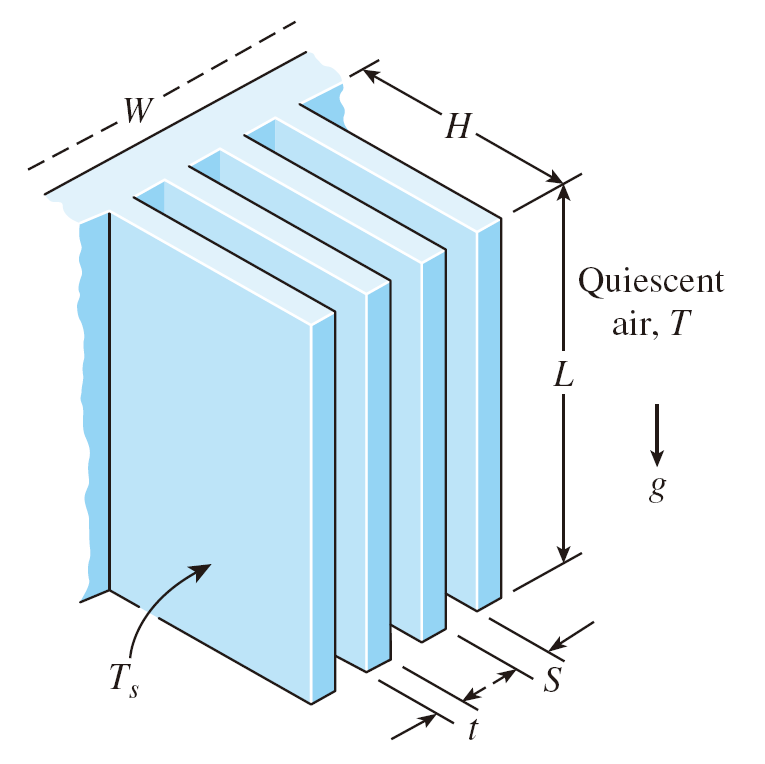
\includegraphics[width=10cm]{fin}
    \caption{fin的尺寸}
\end{figure}

\section{真空系统}
真空系统的气体流动需要使用与传统流体流动问题不同的物理方程来描述。在低压环境下,气体分子的平均自由程与系统的尺度相当,气体的稀薄效应变得很重要。通常情况下,稀薄度可以通过克努森数\footnote{\url{https://en.wikipedia.org/wiki/Knudsen_number}}来描述,分辨真空系统中是使用统计力学还是连续介质假设来描述流体流动。

\begin{equation}\label{Knudsen}
Kn = \frac{\lambda}{L}
\end{equation}

其中$ \lambda $为是气体分子的平均自由程,$ L $为系统的特征尺寸。在动力学理论(kinetic theory)中,分子的平均自由程\footnote{\url{https://en.wikipedia.org/wiki/Mean_free_path}}指分子在与其他分子碰撞之间行进的距离,其中$ k_B $为玻尔兹曼常数,$ d $为分子直径。

\begin{equation}
\lambda = \frac{k_B T}{\sqrt{2}\pi d^2 p}
\end{equation}

\autoref{knudsenVSflow}显示了不同$ Kn $数下的流型及系统适用的控制方程。

\begin{table}[h]
    \centering
    \caption{Knudsen数与流体流动类型}
    \label{knudsenVSflow}
    \begin{tabular}{cc}
        \toprule
        $ Kn $数 & 流动类型 \\
        \midrule
        $ Kn<0.01 $ & 连续介质假设,使用Navier-Stokes方程和传统的计算流体力学方法 \\
        $ 0.01<Kn<0.1 $ & 滑移流,Navier-Stokes方程,壁面处使用\textbf{滑移边界条件}来模拟\textbf{克努森层} \\
        $ 0.1<Kn<10 $ & 过渡流,大部分流体区域都属于克努森层,必须使用稀薄气体动力学方法 \\
        $ Kn>10 $ & 分子流,气体分子只与流体域的表面相互作用,分子之间没有散射现象 \\
        \bottomrule
    \end{tabular}
\end{table}

当$ \lambda<<L $或$ Kn<<0.01 $时,分子之间能发生频繁的碰撞,可视为连续介质。在超高真空系统中,$ \lambda>>L $且$ Kn>10 $,分子之间已经很难发生碰撞,碰撞主要发生在分子和壁之间,属于自由分子流。

\section{高马赫数流动}
马赫数的定义常见维基百科\footnote{\url{https://en.wikipedia.org/wiki/Mach_number}}。马赫数从$ 1.2\sim5.0 $为超音速区,超音速流通过收缩管道时减速、压缩,通过扩散管道时,增速、膨胀。而亚音速流通过收缩管道时,则现象完全相反。

\begin{figure}[h]
    \centering
    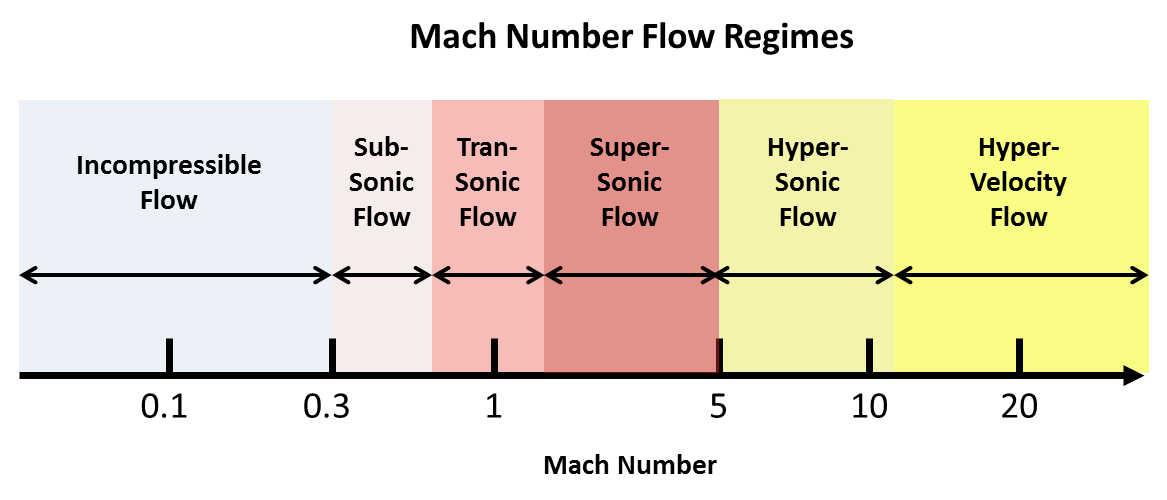
\includegraphics[width=10cm]{Mach-Number-Flow-Regimes}
    \caption{Mach-Number-Flow-Regimes}
\end{figure}

高马赫数流动必须考虑粘性耗散(Viscous dissipation)和压力功(pressure work),模拟高马赫数流动现象必须结合考虑动量和能量传递。在流动过程中热导率$ k $和粘度$ \mu $的变化\textbf{按理想气体}假设来计算。一般使用Sutherland's Law。

\begin{equation}
k = k_{ref}\left( \frac{T}{T_{k,ref}} \right)^{3/2}\frac{T_{k,ref}+S_k}{T+S_k}
\end{equation}

其中,$ k_{ref} $为参考条件下的热导率(\si{\watt\per\meter\per\kelvin}),$ T_{k,ref} $为参考条件下的温度(\si{\kelvin}),$ S_k $为Sutherland常数(\si{\kelvin},每种气体都有自己的常数)。

同理,高马赫流动流体的粘度也可使用Sutherland's Law来计算,\textbf{仅对低压下的单组分气体有效}。

\begin{equation}
\mu = \mu_{ref}\left( \frac{T}{T_{\mu,ref}} \right)^{3/2}\frac{T_{\mu,ref}+S_\mu}{T+S_\mu}
\end{equation}

其中,$ \mu_{ref} $为参考条件下的粘度(\si{\pascal\per\second}),$ T_{\mu,ref} $为参考条件下的温度(\si{\kelvin}),$ S_\mu $为Sutherland常数(\si{\kelvin},每种气体都有自己的常数)。

\section{多孔介质流动}

设多孔介质的基体体积为$ V_s $,孔隙的体积为$ V_f $,整个介质总体积为$ V_m = V_s + V_f $,多孔介质流道所占体积分数为孔隙率$ \varepsilon=V_f/V_m $。

多孔介质单位横截面积(包含孔隙和基体)的体积流率,即在$ V_m $上的平均流速称为\textbf{Darcy速度};在$ V_f $上的平均流速称为\textbf{内在平均速度(The intrinstic average velocity)或孔隙速度(pore velocity)}。

为了使孔隙速度$ u_p $有意义,必须对表征体元(包括孔隙体积和孔隙体积)上的速度进行统计平均,Darcy速度$ u_D $和孔隙速度$ u_p $可以通过Dupuit–Forchheimer relationship进行关联,这个定义使得速度在多孔区域和自由流动区域的边界上连续。

\begin{equation}\label{Dupuit–Forchheimer-relationship}
u_{D} = \varepsilon u_p
\end{equation}

运用通用的守恒方程导出多孔介质流动的连续性方程:

\begin{equation}
\varepsilon \frac{\partial \rho}{\partial t} + \nabla\cdot(\rho\bm{u}) = 0
\end{equation}

Darcy定律表明,流速和压力梯度成正比,流动的阻力主要是流体的粘性力,Darcy适用于低$ Re $的渗流情况。

\begin{equation}\label{Darcy's-law-2D}
u = -\frac{\kappa}{\mu} \frac{\partial p}{\partial x}
\end{equation}

三维情况下,Darcy定律如下式,其中$ \bm{\kappa} $为渗透率张量。

\begin{equation}\label{Darcy's-law-3D}
\bm{u} = -\frac{\bm{\kappa}}{\mu}\cdot\nabla p
\end{equation}

\subsection{渗透率}

流体流过固体基质的水力半径定义为:

\begin{equation}
d_h = \frac{4\times\text{void volume}}{\text{surface area}} = \frac{4\varepsilon}{A_0(1-\varepsilon)}
\end{equation}

其中,$ A_0 $是基于固体体积的比表面积,

\[A_0=\frac{A_{fs}}{V_s}\]

使用曲折因子对压力梯度进行修正,

\begin{equation}
\nabla p_{mod} = \frac{1}{\tau}\nabla p
\end{equation}

其中,曲折因子定义为流动的有效长度$ L_e $和流道进出口直线距离$ L $之比,

\[\tau = \frac{L_e}{L}\]

利用曲折因子$ \tau $和形状参数$ k_0 $来修正Hagen–Poiseuille equation推导的渗流速度,

\begin{equation}
\mathbf{u}_p = \frac{d_h^2}{16k_0\mu\tau}\nabla p
\end{equation}

其中,圆形毛细管的$ k_0=2 $,矩形毛细管的$ k_0=2.0\sim2.5 $,其他形状查阅文献\footnote{Johnson R W. Handbook of fluid dynamics [M]. Crc Press, 2016.}获知。

进一步可对孔隙速度与渗流速度的关联进行修正,

\begin{equation}
\mathbf{u}_D = \mathbf{u}_p\frac{\varepsilon}{\tau} = -\frac{\kappa}{\mu}\nabla p
\end{equation}

求解得到渗透率$ \kappa $,

\begin{equation}
\kappa = \frac{\varepsilon d_h^2}{16k_0\tau^2} =
\frac{\varepsilon d_h^2}{16k_\kappa} = 
\frac{\varepsilon^3}{k_\kappa (1-\varepsilon)^2A_0^2}
\end{equation}

其中,$ k_\kappa = k_0\tau^2 $称为Kozeny constant。

对于任意形状的颗粒,引入等效球体的概念,该颗粒与等效球体具有相同的比表面积,并定义等效球体直径为,

\begin{equation}
d = \frac{6}{A_0}
\end{equation}

对于尺寸均一、直径为$ d_s $的球形来说,$ d=d_s $;对于直径为$ d_c $的圆柱来说,$ d=(3/2)d_c $。

引入等效直径后,渗透率表示为,

\begin{equation}
\boxed{\kappa = \frac{\varepsilon^3}{36k_\kappa(1-\varepsilon)^2}d^2}
\end{equation}

渗透率是由多孔介质几何结构决定的,对于简单和规则的几何结构,我们能够通过几何参数来计算渗透率。比如球形颗粒填充床,渗透率与孔隙率、几何参数有如下关系:

\begin{equation}\label{Carman-Kozeny}
\kappa = \frac{d_p^2\varepsilon^3}{180(1-\varepsilon)^2}
\end{equation}

对于粒径分布较窄的球形填充床,文献提供的预测公式为,

\begin{equation}
\kappa = \frac{\varepsilon^5.5}{5.6}d^2
\end{equation}

\subsection{Forchheimer's Equation}

当Darcy流速$ \bm{u} $足够小(通常意味着$ Re<=1 $),流动符合Darcy定律。随着流速逐渐增大,惯性力带来的非线性曳力逐渐增强,在$ 1<=Re<=10 $这个范围内,惯性力的增长都比较平滑。一旦$ Re $足够高,流动的阻力将主要是流体与流道的摩擦力和惯性力。Forchheimer方程扩展了Darcy定律,适用于多孔介质内的快速流动。大量研究表明,从Darcy流动到Darcy–Forchheimer流动的转变发生在$ Re_{\text{local}}>100 $时。

\begin{equation}\label{Forchheimer}
\nabla p = -\frac{\mu}{\kappa}\bm{u} - c_F \kappa^{-1/2}\rho|\bm{u}|\bm{u}
\end{equation}

其中,$ c_F $为无量纲阻力系数,根据Beavers等人的实验总结,阻力系数可按下式计算:

\begin{equation}
c_F = 0.55 \left( 1-5.5\frac{d}{D_e} \right)
\end{equation}

其中,$ d $为颗粒直径,$ D_e $为床层等效直径,$ D_e=2wh/(w+h) $,$ w $为床层宽度,$ h $为床层高度。

除了Forchheimer方程外,Irmay等人也提出了一个关联多孔介质压降的关联式,当$ \beta=150 $,$ \alpha=1.75 $即为著名的Ergun方程:

\begin{equation}\label{Irmay}
\frac{dp}{dx}=-\frac{\beta\mu(1-\varepsilon)^2 u}{d_p^2\varepsilon^3}-\frac{\alpha\rho(1-\varepsilon)u^2}{d_p\varepsilon^3}
\end{equation}

\subsection{Brinkman's Equation}

\begin{equation}\label{Brinkman}
\rho\left[ \frac{1}{\varepsilon}\frac{\partial \bm{u}}{\partial t} + \frac{1}{\varepsilon}\nabla\left( \frac{\bm{u\cdot u}}{\varepsilon} \right) \right] = -\nabla p + \frac{\mu}{\varepsilon}\nabla^2\bm{u}-\frac{\mu}{\kappa}\bm{u}-\frac{c_F\rho}{\kappa^{1/2}}|\bm{u}|\bm{u}
\end{equation}

\subsection{固定床的压力损失}

通常使用Ergun(1952)和Reichelt(1972)提出的经验关联式来计算压力损失:

\begin{equation}
\frac{\Delta p}{\Delta x} = f\cdot \frac{1}{2} \rho_f \left( \frac{u}{\varepsilon} \right)^2 \frac{1}{d_p}
\end{equation}

其中,速度为Darcy速度,$ f $为摩擦因子,定义为:

\begin{equation}
f = \frac{c_1}{Re_p}+c_2
\end{equation}

一般的关联中$ c_1=133 $,$ c_2=2.33 $。考虑壁面效应的关联中,摩擦因子定义为:

\begin{multline}
f = 2A_w\left( \frac{154A_w}{Re_p} + \frac{1}{B_w} \right) \\
A_w = 1+\frac{2}{3N}(1-\varepsilon) \\
B_w = \left[ 1.15N^2+0.87 \right] \\
N = \frac{d_p}{D}
\end{multline}

\subsection{固定床的孔隙率}
大量实验表明,填充床的孔隙率是一个阻尼振荡函数,从壁面处$ \varepsilon=1 $振荡变化到$ 5d_p $处接近稳定。可用经验公式描述孔隙率的变化:

\begin{equation}
\varepsilon=\varepsilon_{\infty}\left[ 1+C e^{\left(-N\frac{y}{d_p}\right)} \right]
\end{equation}

其中,$ y $是距壁面的距离;$ C $,$ N $是经验参数,实验表明$ C=1.4 $,$ \varepsilon_{\infty}=0.4 $时,$ N=5\ \text{or}\ 6 $。

由于壁面附近孔隙率最大,流动过程中流速也最大,这种现象称为“沟流现象”(channeling effect)。

\section{湍流}








